\documentclass[aspectratio=169,10pt]{beamer}

\usetheme{metropolis}
\usepackage{booktabs}
\usepackage{graphicx}
\usepackage{amsmath}
\usepackage{pifont}
\newcommand{\cmark}{\textcolor{green!55!black}{\ding{51}}}
\newcommand{\xmark}{\textcolor{red!70!black}{\ding{55}}}

\title{GPU-Accelerated Continuous Subgraph Matching}
\subtitle{Why BFS Beats DFS on the SIMT Architecture}
\author{Haibin Lai \and Ziheng Wang \and Rongchuan Li}
\institute{SUSTech HPC Lab}
\date{June 2026}

\begin{document}

\maketitle

% ----------------------------------------------------------------
\begin{frame}{大纲}
\tableofcontents
\end{frame}

% ================================================================
\section{背景与问题}
% ================================================================
\begin{frame}{Continuous Subgraph Matching (CSM)}
  \textbf{任务}：在动态图 $G$ 上，对每个边更新 $\Delta=(v_1,v_2,\ell)$，实时枚举小查询图 $q$ 的所有嵌入。
  \begin{itemize}
    \item \textbf{应用}
    \begin{itemize}
      \item 金融风控 \& 交易图监测 — Bytedance BG3~\cite{zhang2024bg3}
      \item 实时推荐 — Twitter motif detection~\cite{gupta2014twitter}
      \item 网络安全 \& 僵尸网络检测~\cite{lagraa2024network}
    \end{itemize}
    \item \textbf{现有 CPU 系统}：
    GraphFlow~\cite{graphflow},
    TurboFlux~\cite{turboflux},
    SymBi~\cite{rapids-symbi},
    CaLiG~\cite{calig},
    NewSP~\cite{newsp}
    \item \textbf{ParaCOSM (ICPP'25)}~\cite{paracosm2025}：把 5 种算法接到统一执行器，加上两层 CPU 并行
    \begin{itemize}
      \item Inner-update：单条更新内的搜索并行
      \item Inter-update：safe 更新之间的并行
    \end{itemize}
  \end{itemize}
  \vfill
  \alert{瓶颈仍在「单条更新的搜索」本身 → 上 GPU。}
\end{frame}

% ----------------------------------------------------------------
\begin{frame}{形式化定义（沿用 ParaCOSM~\cite{paracosm2025}）}
\begin{columns}[T]
\begin{column}{0.55\textwidth}
\scriptsize
\begin{itemize}
  \item \textbf{标签图}~$g=(V,E)$：带顶点/边标签函数 $L_V,L_E$。
  \item \textbf{匹配 (Def.~2.2)}：$M\!:\!V(Q)\!\to\!V(G)$ 单射，满足标签 \& 邻接约束。
  \item \textbf{图流 (Def.~2.3)}：$\Delta\mathcal{G}=(\Delta G_1,\Delta G_2,\dots)$，每个 $\Delta G=(\pm,e/v)$。
  \item \textbf{CSM 问题 (Def.~2.4)}：对每个 $\Delta G$ 报告\\
        $\Delta\mathcal{M}=\mathcal{M}'\!\triangle\!\mathcal{M}$。
  \item \textbf{Compatible Set (Def.~2.5)}：$C(u,\phi)$ — 下一查询点的可行候选。
\end{itemize}
\end{column}
\begin{column}{0.45\textwidth}
\centering
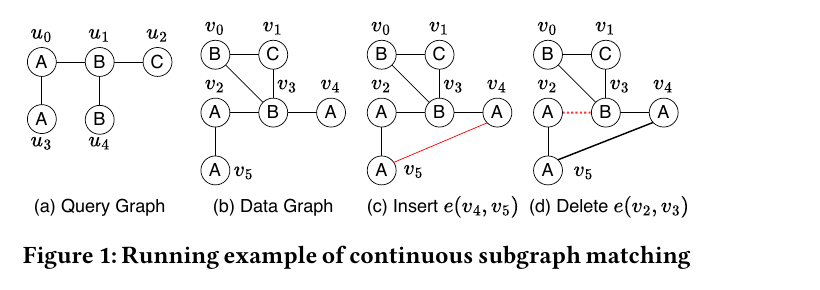
\includegraphics[width=\linewidth]{figures/csm_running_example.png}\\
{\tiny ParaCOSM~\cite{paracosm2025} Fig.~1}
\end{column}
\end{columns}
\end{frame}

% ----------------------------------------------------------------
\begin{frame}{两阶段 CSM 模型 \& Safe / Unsafe 更新}
\begin{columns}[T]
\begin{column}{0.5\textwidth}
\textbf{Offline}
\begin{itemize}
  \item 构建辅助结构~$\mathcal{A}$
  \item 决定匹配顺序~$\mathcal{O}$
  \item 计算初始匹配~$\mathcal{M}_0$
\end{itemize}
\textbf{Online}（每条 $\Delta G$）
\begin{enumerate}
  \item 应用更新 + 维护 $\mathcal{A}$
  \item 以 $e$ 为根、按 $\mathcal{O}$ 展搜索树~$\mathcal{T}$
  \item 枚举 $\Delta\mathcal{M}$
\end{enumerate}
\end{column}
\begin{column}{0.5\textwidth}
\centering
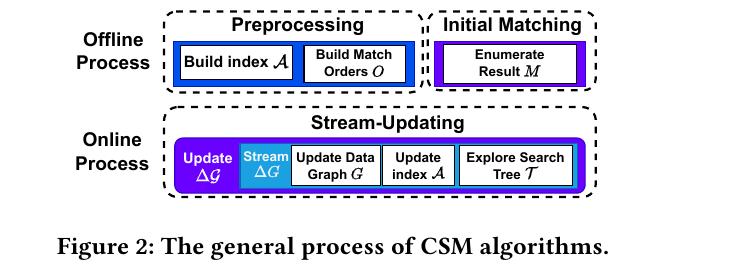
\includegraphics[width=\linewidth]{figures/csm_general_workflow.png}\\
{\tiny ParaCOSM~\cite{paracosm2025} Fig.~2}
\vspace{4pt}

\scriptsize
\textbf{ParaCOSM 关键观察}：$\geq 98.4\%$ 更新为 \emph{safe}；unsafe 触发于 label / degree / candidate 三重过滤。\\
\alert{我们的目标：unsafe 搜索 → GPU。}
\end{column}
\end{columns}
\end{frame}

\begin{frame}{设计抉择：DFS 还是 BFS？}
  \begin{columns}[T]
  \begin{column}{0.5\textwidth}
    \textbf{方案 A：并行 DFS} \\[2pt]
    沿用 CPU 递归，每根独立线程
    \begin{itemize}
      \item \xmark\ 栈指针发散
      \item \xmark\ Hub 顶点尾延迟
      \item \xmark\ 内存访问无规整性
    \end{itemize}
  \end{column}
  \begin{column}{0.5\textwidth}
    \textbf{方案 B：层同步 BFS} \\[2pt]
    一次扩展一层匹配
    \begin{itemize}
      \item \cmark\ Warp 内 lockstep
      \item \cmark\ Prefix-scan 合并写出
      \item \cmark\ 边中心切分易均衡
    \end{itemize}
  \end{column}
  \end{columns}
  \vfill
  \begin{block}{结论}
    在我们尝试的每一对 (algorithm, query) 上，\textbf{BFS 全面胜过 DFS}。本工作的 GPU 路径为 \texttt{gpu\_bfs\_versioned}。
  \end{block}
\end{frame}

% ================================================================
\section{系统设计}
% ================================================================
\begin{frame}{GPU 模块（基于 ParaCOSM 架构）}
  \begin{columns}[T]
  \begin{column}{0.5\textwidth}
  \scriptsize
  \begin{itemize}
    \item \texttt{gpu\_classifier} \hfill \texttt{-m gpu} \\
          边的 safe / unsafe 分类
    \item \texttt{gpu\_candidate\_filter} \hfill PFM2 \\
          相邻 query 顶点的 candidate 过滤
    \item \texttt{gpu\_search} \hfill \texttt{-m gpu\_all} \\
          DFS 风格：每线程一个栈
    \item \texttt{gpu\_bfs\_search} \hfill \texttt{-m gpu\_bfs[\_versioned]} \\
          层同步 BFS，partial-match 驻 device
  \end{itemize}
  \textbf{Versioned}：部分匹配挂时间戳，多条 unsafe 共用一次 BFS。
  \end{column}
  \begin{column}{0.5\textwidth}
  \centering
  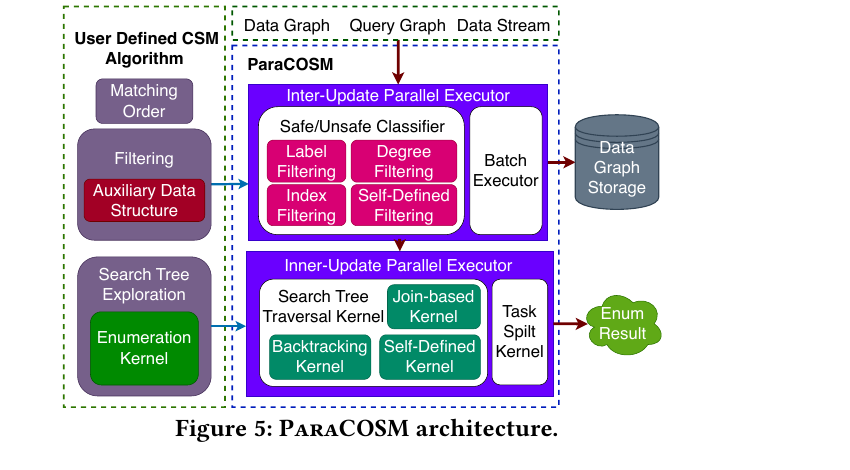
\includegraphics[width=\linewidth]{figures/csm_paracosm_arch.png}\\
  {\tiny ParaCOSM~\cite{paracosm2025} Fig.~5；GPU 后端替换 Inter-/Inner-Update Executor。}
  \end{column}
  \end{columns}
\end{frame}

\begin{frame}{Versioned BFS：核心想法}
  \begin{enumerate}
    \item 把当前批次中所有 unsafe 更新的根 $(v_1,v_2)$ 一起放入 frontier。
    \item 每条 partial-match 携带 \texttt{ver\_id}（属于哪条更新）。
    \item 每层扩展：所有线程对同一 query 顶点做 join + filter。
    \item 写出阶段：prefix-scan 计算偏移，coalesced 写入 partial-match buffer。
    \item Buffer 满 → flush 到结果计数。
  \end{enumerate}
  \vfill
  \alert{关键好处}：分类 / 边插入 / CSR 构造的固定开销，被一次 BFS 摊销给整个 batch。
\end{frame}

% ================================================================
\section{主实验：Amazon (AZ) 8v}
% ================================================================
\begin{frame}{实验配置}
  \begin{columns}
  \begin{column}{0.55\textwidth}
    \textbf{硬件}
    \begin{itemize}
      \item A100-SXM4-80GB $\times$ 1
      \item Xeon Platinum 8470, 96 核
      \item 1.7 TB DRAM
    \end{itemize}
    \textbf{软件}
    \begin{itemize}
      \item oneAPI 2025.3 (icpx)
      \item CUDA 12.9, sm\_80
    \end{itemize}
  \end{column}
  \begin{column}{0.45\textwidth}
    \textbf{数据 \& 工作负载}
    \begin{itemize}
      \item AZ：$|V|\!\approx\!0.4$M, $|E|\!\approx\!3.4$M
      \item LJ：$|V|\!\approx\!4.85$M, $|E|\!\approx\!38.6$M
      \item 100 个 8-顶点查询
      \item 1800\,s timeout / pair
    \end{itemize}
    \textbf{基线}：CPU \texttt{-m single -t 1}
  \end{column}
  \end{columns}
\end{frame}

\begin{frame}{AZ 8v：5 种算法的中位加速比}
  \centering
  \begin{tabular}{lr}
    \toprule
    \textbf{算法} & \textbf{中位加速比} \\
    \midrule
    \textsc{Parallel\_NewSP}      & $\mathbf{51.1\times}$ \\
    \textsc{Parallel\_TurboFlux}  & $49.5\times$ \\
    \textsc{Parallel\_GraphFlow}  & $46.5\times$ \\
    \textsc{Parallel\_SymBi}      & $25.3\times$ \\
    \textsc{Parallel\_CaLiG}      & $21.7\times$ \\
    \bottomrule
  \end{tabular}
  \vfill
  \footnotesize
  CaLiG 加速比偏低：CPU 端已维护 candidate-set 索引，绝对 CPU 时间小，PCIe + kernel-launch 固定开销占比上升。
\end{frame}

\begin{frame}{AZ 8v：分布图}
  \centering
  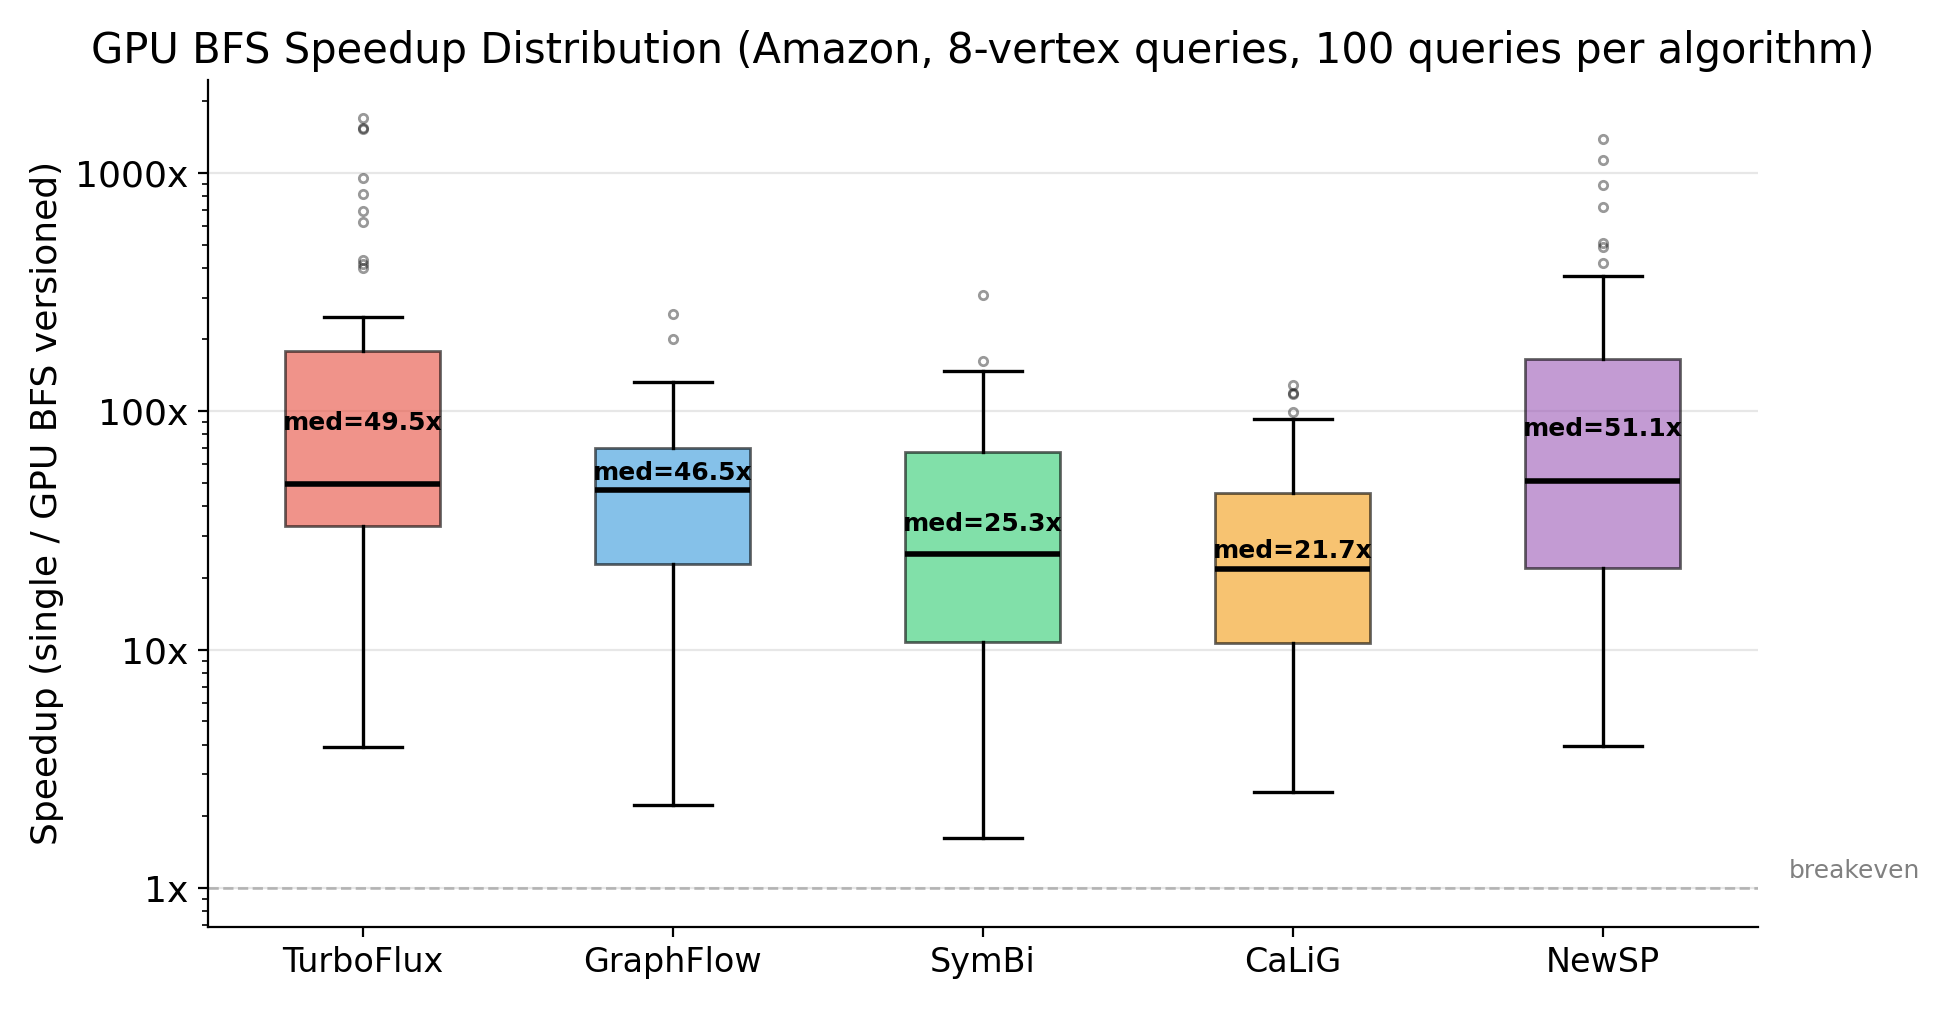
\includegraphics[width=0.85\textwidth]{figures/speedup_8v_by_algo.png}
\end{frame}

\begin{frame}{BFS 视角的搜索树 — AZ Q\_5 (GraphFlow)}
  \centering
  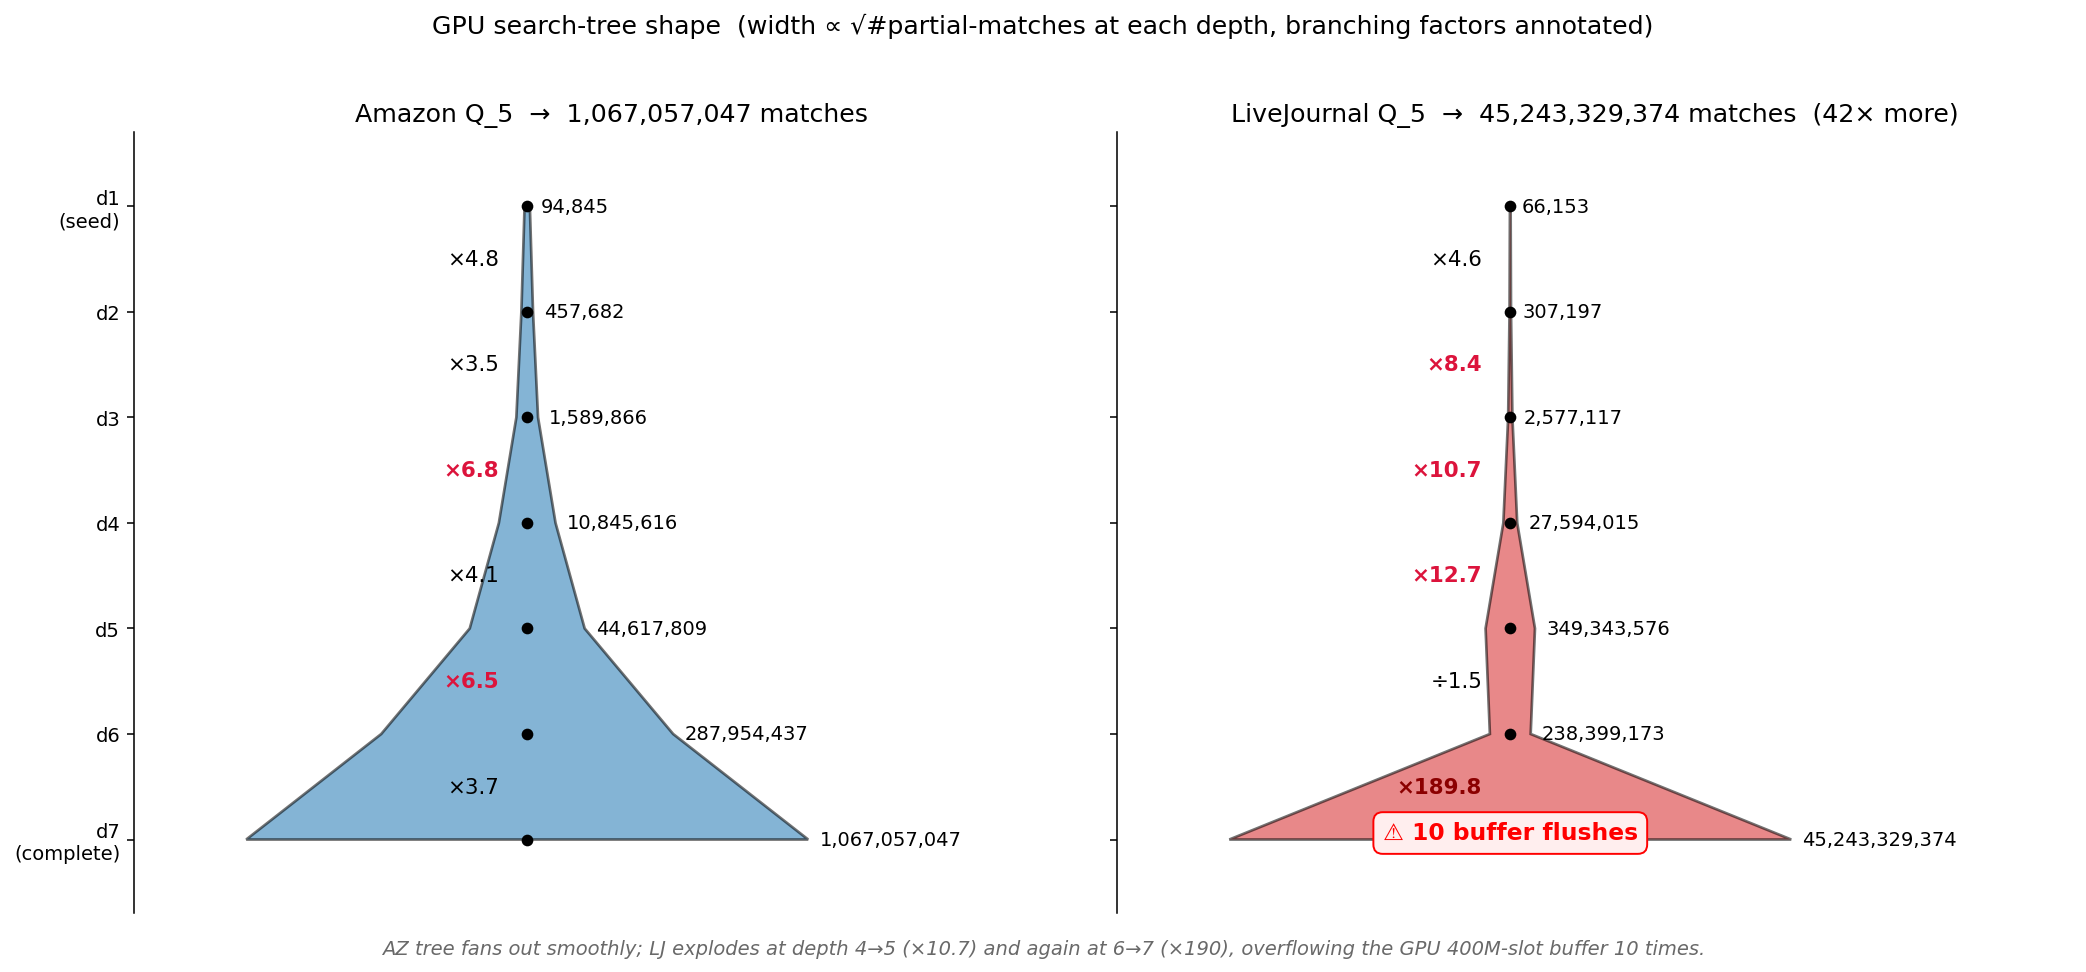
\includegraphics[width=0.85\textwidth]{figures/bfs_tree_q5_silhouette.png}\\[4pt]
  \footnotesize
  中间层 (depth 4--5) 是负载均衡的关键区。\\
  最大 partial-match 数稳稳低于 $4\times10^8$ 设备 buffer，BFS 全程 \emph{不需要 flush}。
\end{frame}

% ================================================================
\section{边界情形：LiveJournal}
% ================================================================
\begin{frame}{LJ 8v：picture turns mixed}
  \centering
  \small
  \begin{tabular}{lrrrr}
    \toprule
    \textbf{算法} & \textbf{pairs} & \textbf{cpu (s)} & \textbf{gpu (s)} & \textbf{加速} \\
    \midrule
    \textsc{GraphFlow} &  1 & 1494.6 &  105.4 & $14.18\times$ \\
    \textsc{TurboFlux} &  9 &  666.3 &  215.2 & $3.10\times$  \\
    \textsc{CaLiG}     & 14 &  583.6 &  658.9 & $0.89\times$  \\
    \textsc{NewSP$^*$} & 16 &   87.1 &  637.0 & $0.14\times$  \\
    \textsc{SymBi}     &  0 & --- & --- & ---           \\
    \bottomrule
  \end{tabular}
  \vfill
  \footnotesize
  $^*$\textsc{NewSP} 的 CPU \texttt{single} 路径返回 0 个匹配（adapter stub）— 见下页。
\end{frame}

\begin{frame}[fragile]{NewSP CPU stub：被发现的实现 bug}
\begin{verbatim}
size_t Parallel_NewSP_Adapter::EnumerateNewEdge(
        uint v1, uint v2, uint label, size_t /*tid*/) {
  // Not implemented for NewSP adapter -- use versioned mode
  return 0;
}
\end{verbatim}
  \vfill
  \begin{itemize}
    \item CPU \texttt{single} 不做实际 matching → CPU 假性「跑得快」
    \item 其它 4 个算法 GPU 与 CPU 计数到 7 位有效数字一致 → BFS 实现\textbf{正确}
    \item 公平比较需要 CPU \texttt{-m versioned}（正在跑）
  \end{itemize}
\end{frame}

\begin{frame}{LJ 上发生了什么：搜索空间爆炸}
  \centering
  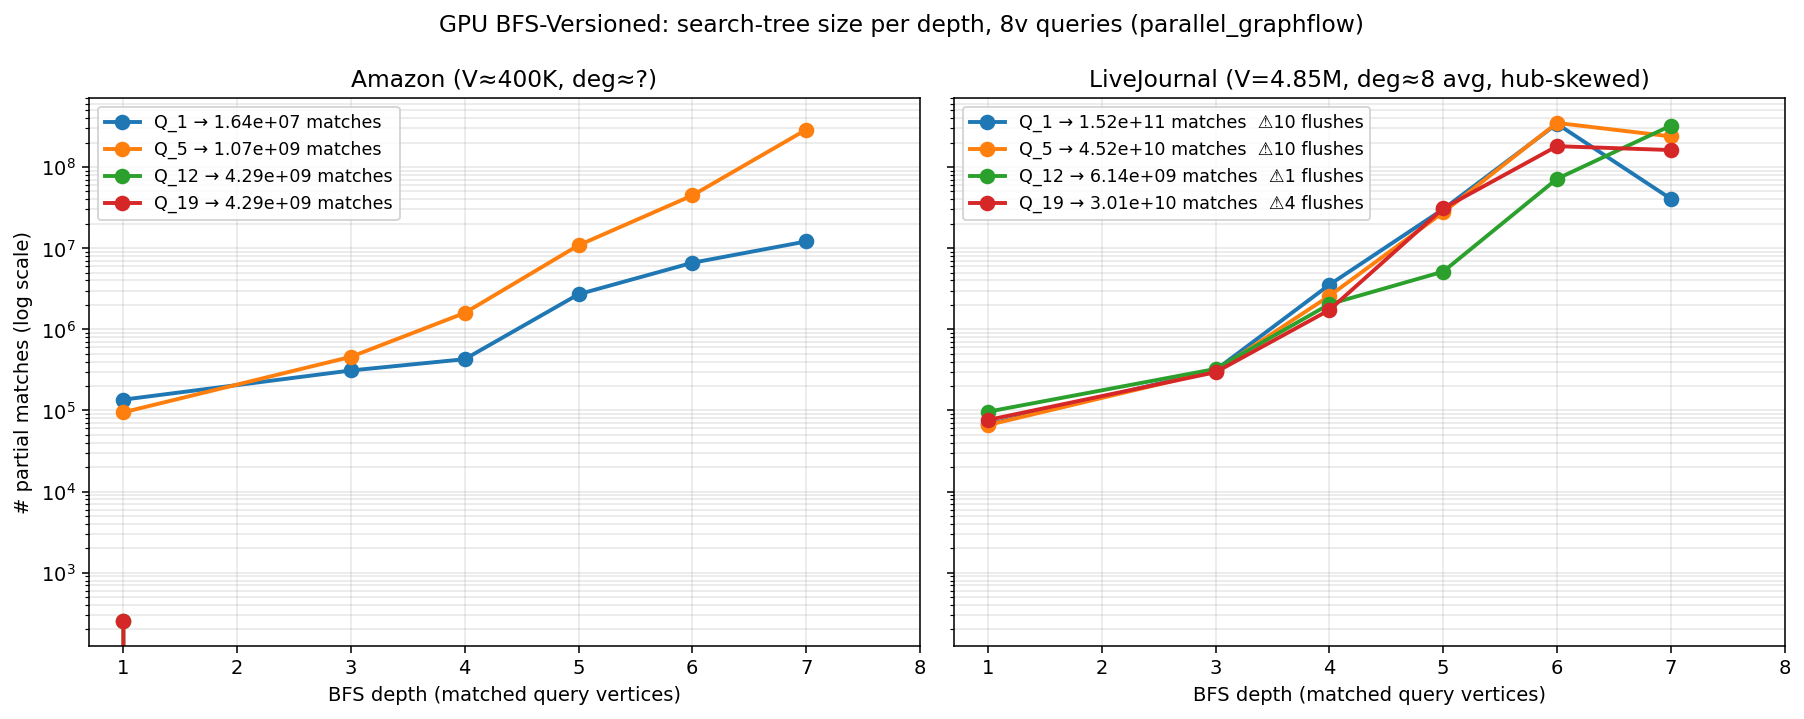
\includegraphics[width=0.78\textwidth]{figures/bfs_tree_az_vs_lj.png}\\[4pt]
  \footnotesize
  LJ 中间层每一层都比 AZ 高一个数量级。\\
  LJ \textsc{NewSP} \texttt{Q\_19}：$7.97\times10^{10}$ 匹配，partial-match buffer \textbf{flush 15 次}。
\end{frame}

\begin{frame}[fragile]{典型 log 片段}
\begin{verbatim}
[BFS-V] Depth 5->6: 4.83e7 -> 3.85e8
[BFS-V] Flush 400000000 partials at depth 6->7  (x15)
Search complete: 7.97e10 matches, 1019.0 s
\end{verbatim}
\vfill
\begin{block}{诊断}
瓶颈不是算力，是 \textbf{固定大小的 device buffer}。每次 flush 都把整个 BFS 流水线 stall 住。
\end{block}
\end{frame}

% ================================================================
\section{改进方向}
% ================================================================
\begin{frame}{Short-term：可立刻动手的}
  \begin{itemize}
    \item \textbf{Edge-centric 工作切分}\\
          binary-search row-split，每线程负责均匀的边，消除 hub 尾延迟
    \item \textbf{Partial-match streaming}\\
          buffer 满时把溢出部分 D2H 拷到 pinned memory；下一层 BFS 与拷贝 \emph{并行}\\
          → 直接缓解 LJ flush thrashing
    \item \textbf{H2D / search overlap}\\
          边插入走独立 stream，不再阻塞 BFS
  \end{itemize}
\end{frame}

\begin{frame}{Medium-term：自适应与剪枝}
  \begin{itemize}
    \item \textbf{自适应 DFS $\leftrightarrow$ BFS}\\
          候选集小时，BFS 启动开销占比高 → 退化到 DFS\\
          决策依据：query 拓扑 + 第一层 BFS 的候选数
    \item \textbf{Early intersection pruning}\\
          在 partial-match \emph{发射} 时就做 backward-neighbor 交集，\\
          而不是等到下一层 BFS。LJ 上中间层冗余很大，受益最大。
  \end{itemize}
\end{frame}

\begin{frame}{Long-term：多 GPU \& CPU/GPU 混合}
  \begin{itemize}
    \item \textbf{多 GPU}
    \begin{itemize}
      \item Query 维度切分：每 GPU 一组 query（耦合弱）
      \item Update 维度切分：safe-update batch 切给不同 GPU
    \end{itemize}
    \item \textbf{CPU / GPU 混合}
    \begin{itemize}
      \item Safe update → CPU；unsafe → GPU
      \item 前提：补齐 \textsc{NewSP} 的 CPU \texttt{versioned} 实现
      \item 让算法放置成为 data-driven 的决策
    \end{itemize}
  \end{itemize}
\end{frame}

% ================================================================
\section{总结}
% ================================================================
\begin{frame}{Take-aways}
  \begin{enumerate}
    \item GPU 上做 CSM，\textbf{层同步 BFS} 比并行 DFS 全面更优。
    \item AZ 8v：BFS-versioned 在 5 种 SOTA 算法上拿到 \textbf{$21\times$ — $51\times$} 中位加速。
    \item LJ 上瓶颈\emph{可被定位}：固定大小 device buffer 引发的 H2D flush。
    \item 用「逐层 partial-match 计数」做 profiling，方法可推广到其它\\GPU graph mining workload。
  \end{enumerate}
  \vfill
  \centering
  \alert{\Large 谢谢！}\\[6pt]
  \footnotesize
  代码：ParaCOSM, branch \texttt{feat/gpu-profiling-charts}\\
  报告 \& 数据：\texttt{docs/gpu\_csm\_report/}
\end{frame}

% ----------------------------------------------------------------
\begin{frame}[allowframebreaks]{参考文献}
  \tiny
  \bibliographystyle{plain}
  \bibliography{report}
\end{frame}

\end{document}
